\definecolor{singleShotColor}{RGB}{196,106,28}
\definecolor{pipelineColor}{RGB}{44,138,100}
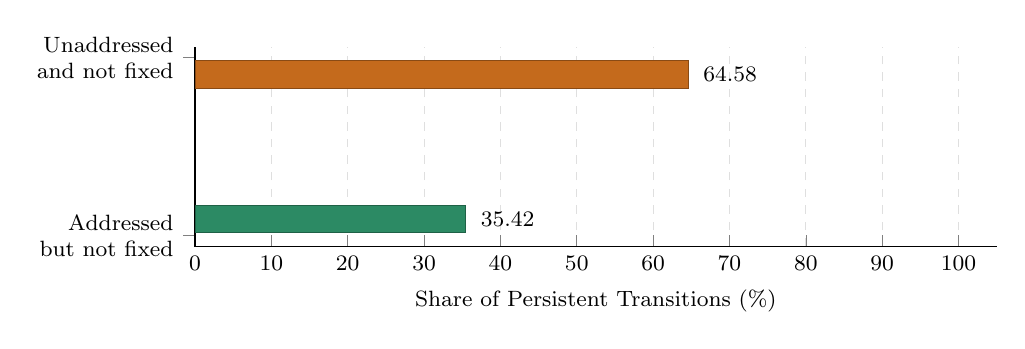
\begin{tikzpicture}
\begin{axis}[
    xbar,
    width=0.97\columnwidth,
    height=0.34\columnwidth,
    xmin=0,
    xmax=105,
    xlabel={Share of Persistent Transitions (\%)},
    symbolic y coords={Addressed,Unaddressed},
    ytick={Unaddressed,Addressed},
    yticklabels={{Unaddressed\\and not fixed},{Addressed\\but not fixed}},
    enlarge y limits={abs=4pt},
    axis lines*=left,
    xmajorgrids=true,
    grid style={dashed,gray!25},
    tick label style={font=\footnotesize},
    yticklabel style={align=right},
    label style={font=\footnotesize},
    nodes near coords={\pgfmathprintnumber[fixed,precision=2]{\pgfplotspointmeta}},
    every node near coord/.append style={font=\footnotesize, text=black, anchor=west, xshift=2pt},
]
\addplot+[fill=singleShotColor, draw=singleShotColor!70!black] coordinates {
    (64.58,Unaddressed)
};
\addplot+[fill=pipelineColor, draw=pipelineColor!70!black] coordinates {
    (35.42,Addressed)
};
\end{axis}
\end{tikzpicture}
